\documentclass[aspectratio=169,10pt]{beamer}
\usepackage[T1]{fontenc}
\usepackage{lmodern,amsmath,amssymb,bm,booktabs,array,graphicx,tikz}
\usetikzlibrary{arrows.meta,positioning,calc,fit}
\definecolor{navy}{HTML}{18334D}
\definecolor{blue}{HTML}{35577F}
\definecolor{teal}{HTML}{158371}
\definecolor{orange}{HTML}{DF9008}
\definecolor{muted}{HTML}{536473}
\definecolor{pale}{HTML}{EFF4F7}
\definecolor{paleteal}{HTML}{E9F5F1}
\definecolor{paleorange}{HTML}{FCF2DF}
\setbeamercolor{normal text}{fg=navy,bg=white}
\setbeamercolor{structure}{fg=teal}
\setbeamercolor{frametitle}{fg=navy}
\setbeamercolor{block title}{fg=navy,bg=pale}
\setbeamercolor{block body}{fg=navy,bg=pale!65}
\setbeamercolor{alerted text}{fg=orange}
\setbeamerfont{frametitle}{size=\large,series=\bfseries}
\setbeamersize{text margin left=7mm,text margin right=7mm}
\setbeamertemplate{navigation symbols}{}
\setbeamertemplate{itemize item}{\color{teal}\small$\bullet$}
\setbeamertemplate{itemize subitem}{\color{teal}\tiny$\bullet$}
\setbeamertemplate{frametitle}{\vspace{2mm}\insertframetitle\par\vspace{1.5mm}\textcolor{teal}{\rule{\textwidth}{0.65pt}}\vspace{-2mm}}
\setbeamertemplate{footline}{\leavevmode\hbox{\begin{beamercolorbox}[wd=.79\paperwidth,ht=2.6ex,dp=1.2ex,leftskip=7mm]{normal text}\scriptsize\color{muted}PassengerAn\quad\textbar\quad SPRING for FQHE\quad\textbar\quad 12 November 2026\end{beamercolorbox}\begin{beamercolorbox}[wd=.21\paperwidth,ht=2.6ex,dp=1.2ex,rightskip=7mm plus1fil]{normal text}\hfill\scriptsize\color{muted}\insertframenumber\,/\,\inserttotalframenumber\end{beamercolorbox}}}
\setlength{\abovedisplayskip}{5pt}
\setlength{\belowdisplayskip}{5pt}
\setlength{\tabcolsep}{5pt}
\hypersetup{colorlinks=true,urlcolor=teal,linkcolor=teal,pdftitle={SPRING for fractional quantum Hall wavefunctions},pdfauthor={PassengerAn}}
\pdfstringdefDisableCommands{\def\translate#1{#1}}
\graphicspath{{support/figures/}}
\newcommand{\src}[1]{\vfill{\fontsize{6.3}{7.5}\selectfont\color{muted}#1\par}}
\newcommand{\take}[1]{\vspace{1mm}\begin{beamercolorbox}[sep=1.6mm,wd=\textwidth]{block body}\small\color{teal}\textbf{#1}\end{beamercolorbox}}
\newcommand{\ml}[1]{{\color{teal}\textbf{ML:} #1}}
\newcommand{\E}{\mathbb E}
\newcommand{\R}{\mathbb R}
\newcommand{\ket}[1]{\lvert #1\rangle}
\newcommand{\bra}[1]{\langle #1\rvert}
\newcommand{\nn}{\mathbf n}
\newcommand{\dO}{\delta O}
\newcommand{\de}{\delta e}
\newcommand{\fidelity}{\mathcal F}
\newcolumntype{L}[1]{>{\raggedright\arraybackslash}p{#1}}
\title{SPRING for fractional quantum Hall wavefunctions}
\author{PassengerAn}
\date{12 November 2026}
\begin{document}

% 1
\begin{frame}[plain]
\vspace{5mm}
{\color{teal}\small VARIATIONAL QUANTUM STATES\quad /\quad PHYSICS + MACHINE LEARNING}\par
\vspace{5mm}
{\fontsize{26}{31}\selectfont\bfseries SPRING for fractional\\quantum Hall wavefunctions}\par
\vspace{5mm}
{\large Haldane sphere, neural coefficients, and the sampling bottleneck}\par
\vspace{7mm}
\begin{columns}[T,onlytextwidth]
\column{.31\textwidth}\textbf{Physics}\par\small LLL basis, pair interactions, and a projected edge potential.
\column{.31\textwidth}\textbf{Optimization}\par\small VMC $\rightarrow$ SR/MinSR $\rightarrow$ projected direction memory.
\column{.31\textwidth}\textbf{Evidence}\par\small Ising validation, FQHE accuracy limits, and broader-pool tests.
\end{columns}
\vfill
{\small PassengerAn\quad\textbar\quad 12 November 2026}\par
{\scriptsize\color{muted}21 main slides + 2 reference/technical backup slides. Numerical results are saved project calculations.}
\end{frame}

\section{Physics model}
% 2
\begin{frame}{The Haldane sphere gives a finite, symmetry-aware LLL}
\begin{columns}[T,onlytextwidth]
\column{.48\textwidth}
\includegraphics[width=.9\linewidth,height=5.0cm,keepaspectratio]{haldane_sphere_wall.pdf}
\column{.50\textwidth}
\begin{itemize}\setlength\itemsep{3pt}
\item Monopole flux $N_\phi=2Q$; sphere radius $R_s=\sqrt Q\,\ell_B$.
\item LLL monopole harmonics have $\ell=Q$, $m=-Q,\ldots,Q$ and $N_{\rm orb}=2Q+1$:
\[
\varphi_m(u,v)\propto u^{Q+m}v^{Q-m}.
\]
\small Spinors satisfy $|u|^2=1-x$, $|v|^2=x$.
\item At the Laughlin $1/3$ shift,
\[N_\phi=3(N_e-1).\]
\item Current test: $N_e=7$, $N_\phi=18$, $Q=9$; \textbf{19 orbitals}.
\end{itemize}
\end{columns}
\take{LLL projection fixes the single-particle space; the network still has to learn the many-body state.}
\src{[1,2] Haldane and Laughlin. Kinetic energy is a constant in the retained LLL; Landau-level mixing is neglected. $N_e/(N_\phi+1)$ is not exactly $1/3$ at finite size.}
\end{frame}

% 3
\begin{frame}{Represent the state by coefficients of Slater determinants}
\begin{columns}[T,onlytextwidth]
\column{.58\textwidth}
\[
\ket{\nn}=(c^\dagger_{-Q})^{n_{-Q}}\cdots(c^\dagger_Q)^{n_Q}\ket0,
\qquad n_m\in\{0,1\}.
\]
\[
\ket{\Psi_\theta}=\sum_{\nn\in\mathcal B_{N_e,M}}\psi_\theta(\nn)\ket{\nn}.
\]
\begin{itemize}\setlength\itemsep{5pt}
\item Canonical creation-operator order enforces fermionic antisymmetry.
\item Fix $\sum_m n_m=N_e$ and $\sum_m m n_m=M=L_z$.
\item Current sector: $M=0$, dimension \textbf{1,656}.
\item $L_z=0$ does not impose $L^2=0$.
\end{itemize}
\column{.38\textwidth}
\begin{block}{One network query}
\small
\textbf{Input:} one binary occupation array\\
$\nn=(n_{-9},\ldots,n_9)\in\{0,1\}^{19}$.\par\medskip
\textbf{Output:} one complex coefficient $\psi_\theta(\nn)$.\par\medskip
It labels an entire many-electron configuration, rather than a single orbital.
\end{block}
\ml{physics restricts the allowed input space.}
\end{columns}
\src{Implementation: physics.py (canonical masks and pair-hop signs), legacy\_model.py (occupation-coefficient network). ED enumerates the sector only for benchmarks/evaluation.}
\end{frame}

% 4
\begin{frame}{The interaction penalizes pairs with relative angular momentum one}
\begin{columns}[T,onlytextwidth]
\column{.58\textwidth}
\[
H_{\rm int}=\sum_{i<j}\sum_{R\;\mathrm{odd}}V_R\,\mathcal P_{ij}^{(R)},
\qquad L_{ij}=2Q-R.
\]
\[
\boxed{\ H_{\rm int}/V_1=\sum_{i<j}\mathcal P_{ij}^{(R=1)}\ }
\]
\begin{itemize}\setlength\itemsep{5pt}
\item $R$ is pair relative angular momentum; odd $R$ is allowed for polarized fermions.
\item The code builds normalized pair projectors in each two-particle $L_z$ block.
\item Pair hopping changes occupations while preserving total $N_e$ and $L_z$.
\end{itemize}
\column{.38\textwidth}
\begin{block}{A known physical target}
At $N_\phi=3(N_e-1)$ with no wall, the Laughlin state has no $R=1$ pairs:
\[H_{V_1}\ket{\Psi_{\rm L}}=0.\]
Its coefficients are \textbf{not supplied} to the network.
\end{block}
\small This is a parent-Hamiltonian test, rather than the full Coulomb interaction.
\end{columns}
\take{Domain knowledge specifies the Hamiltonian and basis, without inserting the ground-state answer into the ansatz.}
\src{[1,2]. physics.py: pair-projector construction from two-particle $L^2$ and exact canonical fermion signs. Energies are in units of normalized $V_1$.}
\end{frame}

% 5
\begin{frame}{Add a finite spatial wall, then project it into the LLL}
\begin{columns}[T,onlytextwidth]
\column{.52\textwidth}
\[
x=\sin^2(\vartheta/2),\qquad U(x)=U\,\Theta(x-x_c),
\]
\[
H=H_{V_1}+\sum_{m=-Q}^{Q}\epsilon_m n_m,\quad
\epsilon_m=\bra{Qm}\widehat U(x)\ket{Qm}.
\]
{\small With $a=m+Q$, $F=2Q$, and $k=F-a$,}
\[
\epsilon_a=U\!\int_{x_c}^{1}\!\frac{x^k(1-x)^{F-k}}{B(k+1,F-k+1)}\,dx.
\]
\small Current choice: $U=10V_1$, $x_c=0.88$; all 19 orbitals remain.
\column{.46\textwidth}
\includegraphics[width=\linewidth]{projected_wall_profile.pdf}
\small The southern 12\% of sphere area is penalized; LLL projection smooths the orbital energies.
\end{columns}
\take{The sphere has no physical boundary. This wall preserves $L_z$, breaks full rotational symmetry, and changes the ground state.}
\src{north\_droplet.py: beta-distribution survival integral, not an orbital cutoff. For this fixed $N_e=7,L_z=0$ wall Hamiltonian, ED gives $E_0=2.823084663V_1$; no $L^2$ penalty is used.}
\end{frame}

\section{VMC and SPRING}
% 6
\begin{frame}{The physical energy is the loss for every network depth}
\[
\mathcal L(\theta)=E(\theta)=
\frac{\bra{\Psi_\theta}H\ket{\Psi_\theta}}{\langle\Psi_\theta|\Psi_\theta\rangle}
=\E_{p_\theta}\!\left[E_{\rm loc}(\nn)\right],\quad
p_\theta(\nn)=\frac{|\psi_\theta(\nn)|^2}{\sum_{\nn'}|\psi_\theta(\nn')|^2}.
\]
\[
E_{\rm loc}(\nn)=\sum_{\nn'}H_{\nn\nn'}\,
\exp\!\left[\log\psi_\theta(\nn')-\log\psi_\theta(\nn)\right].
\]
\begin{columns}[T,onlytextwidth]
\column{.48\textwidth}
\begin{block}{Physics supplies the calculation}
Interaction: sum coefficient ratios over allowed pair hops.\par\smallskip
Wall: add the diagonal value $\sum_m\epsilon_m n_m$.
\end{block}
\column{.48\textwidth}
\begin{block}{ML learns the variational parameters}
No ground-state labels are required.\par\smallskip
Samples change as the network changes: this is not a fixed training dataset.
\end{block}
\end{columns}
\take{VMC is the sampling-and-estimation framework; SGD, MinSR and SPRING are optimizer choices inside it.}
\src{[3--5]. Code local\_energy.py and north\_droplet.py apply the known Hamiltonian; ED eigenvectors enter only independent validation. Exact energy is real although finite-sample local-energy means may have an imaginary part.}
\end{frame}

% 7
\begin{frame}{From the energy gradient to a sample-space geometric solve}
\small Let $\widehat f=A^Te$ estimate $\tfrac12\nabla_\theta E$ and $\widehat S=A^TA$ estimate the real-parameter quantum metric.
\vspace{2mm}
\renewcommand{\arraystretch}{1.2}
\begin{tabular}{@{}L{.16\textwidth}L{.43\textwidth}L{.33\textwidth}@{}}
\toprule
Method & Direction / operation & Effect\\\midrule
SGD & $\Delta\theta=-2\eta\widehat f$ & No geometric preconditioner.\\
SR & $d=(\widehat S+\lambda I)^{-1}\widehat f$ & Wavefunction geometry; primal solve is $P\times P$.\\
MinSR & $d=A^T(AA^T+\lambda I)^{-1}e$ & Smaller dual solve when $B\ll P$.\\
SPRING & Correct $\mu d_{k-1}$ with the current batch & Reuses compatible past information.\\\bottomrule
\end{tabular}\par
\vspace{2mm}
\small $e$ is the centered local energy in realified sample space. All geometric directions are applied with a minus sign.
\take{MinSR reduces the solve dimension; SPRING addresses the information discarded when each small-batch solve starts from zero.}
\src{[4,5]. Conceptual dense costs: primal metric $P\times P$, minimal complex-state dual $2B\times2B$. Jacobian evaluation and Gram construction still cost time; no general exponential speedup is claimed.}
\end{frame}

% 8
\begin{frame}{SPRING corrects a previous direction using the current batch}
\[
\boxed{d_k=\mu d_{k-1}+A_k^T(A_kA_k^T+\lambda I)^{-1}
\left(e_k-A_k\mu d_{k-1}\right)}
\]
\begin{columns}[T,onlytextwidth]
\column{.58\textwidth}
\begin{enumerate}\setlength\itemsep{6pt}
\item Retain a decayed previous direction $\mu d_{k-1}$.
\item Measure its mismatch with the current sampled equations.
\item Correct the observed component; retain the unseen component.
\end{enumerate}
\small $\mu=0$ recovers damped MinSR. Old Jacobians are not stored.
\column{.38\textwidth}
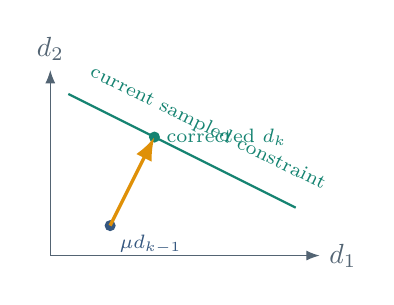
\begin{tikzpicture}[x=.76cm,y=.76cm,>=Latex]
\draw[->,muted] (0,0)--(4.5,0) node[right]{$d_1$};
\draw[->,muted] (0,0)--(0,3.1) node[above]{$d_2$};
\draw[teal,thick] (.3,2.7)--(4.1,.8);
\node[teal,above,rotate=-26] at (2.5,1.85) {\scriptsize current sampled constraint};
\fill[blue] (1,.5) circle(2pt) node[below right]{\scriptsize $\mu d_{k-1}$};
\fill[teal] (1.74,1.98) circle(2pt);
\draw[->,orange,very thick] (1,.5)--(1.74,1.98);
\node[teal,right] at (1.78,1.97) {\scriptsize corrected $d_k$};
\end{tikzpicture}
\end{columns}
\begin{beamercolorbox}[sep=1.5mm,wd=\textwidth]{block body}\small
\textbf{Original-paper evidence:} tuned FermiNet oxygen tests reached chemical accuracy at 40k SPRING updates; MinSR/KFAC did not by 100k. This is a molecular benchmark, not our FQHE comparison.
\end{beamercolorbox}
\src{[5], Sec. 3 and Fig. 2. Figure is schematic: exact projection requires $\lambda=0$ and consistent equations; our damped, changing nonlinear problem has no classical Kaczmarz convergence guarantee.}
\end{frame}

\section{Network and training}
% 9
\begin{frame}{Two real heads describe one complex many-body coefficient}
\begin{columns}[T,onlytextwidth]
\column{.58\textwidth}
\[
\nn\in\{0,1\}^{19}\ \longmapsto\ x=2\nn-1
\ \longmapsto\ (a_\theta(\nn),\varphi_\theta(\nn)).
\]
\[
\boxed{\psi_\theta(\nn)=e^{a_\theta(\nn)+i\varphi_\theta(\nn)}}
\]
\[
\Re\psi=e^a\cos\varphi,\qquad \Im\psi=e^a\sin\varphi.
\]
\begin{itemize}\setlength\itemsep{6pt}
\item $a$ controls relative configuration probabilities: $p_\theta\propto e^{2a}$.
\item $\varphi$ controls coefficient interference in local-energy ratios and expectation values.
\end{itemize}
\column{.38\textwidth}
\begin{block}{Interpretation}
\small
The heads output \textbf{log magnitude and phase}, not raw real/imaginary coefficients.\par\medskip
$\theta$ is the collection of network weights and biases.\par\medskip
$\nn$ is a whole Fock configuration, not an orbital index.
\end{block}
\ml{one nonlinear regressor with two real-valued heads.}
\end{columns}
\src{legacy\_model.py: log\_psi and score\_tree. All trainable parameters are real. This occupation-space MLP is different from the real-space, LL-mixing disk FNN in [6].}
\end{frame}

% 10
\begin{frame}{Every hidden layer contributes to the final readout}
\[
h^{(1)}=\tanh(xW^{(1)}+b^{(1)}),\qquad
h^{(\ell)}=\tanh(h^{(\ell-1)}W^{(\ell)}+b^{(\ell)}),
\]
\[
\boxed{(a_\theta,\varphi_\theta)=c+\sum_{\ell=1}^{6}h^{(\ell)}R^{(\ell)}}.
\]
\begin{center}\vspace{-1mm}
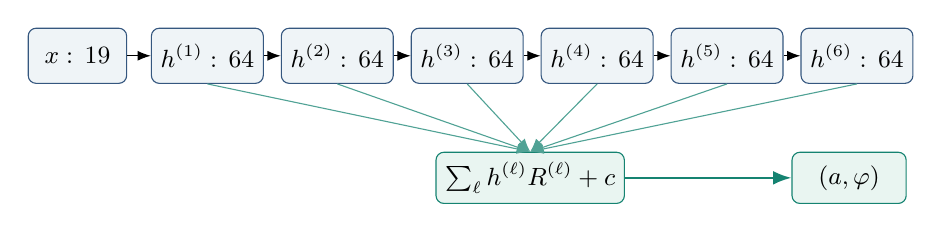
\begin{tikzpicture}[x=1cm,y=1cm,>=Latex,
layer/.style={draw=blue,fill=pale,rounded corners=1mm,minimum width=1.25cm,minimum height=.7cm,font=\small},
head/.style={draw=teal,fill=paleteal,rounded corners=1mm,minimum width=1.45cm,minimum height=.65cm,font=\small}]
\node[layer] (x) at (0,0) {$x:\,19$};
\foreach \i in {1,...,6}{\node[layer] (h\i) at (1.65*\i,0) {$h^{(\i)}:\,64$};}
\draw[->] (x)--(h1);\foreach \i/\j in {1/2,2/3,3/4,4/5,5/6}{\draw[->] (h\i)--(h\j);}
\node[head] (sum) at (5.75,-1.55) {$\sum_\ell h^{(\ell)}R^{(\ell)}+c$};
\foreach \i in {1,...,6}{\draw[->,teal!75] (h\i.south)--(sum.north);}
\node[head] (out) at (9.8,-1.55) {$(a,\varphi)$};\draw[->,teal,thick] (sum)--(out);
\end{tikzpicture}
\end{center}
\begin{itemize}\setlength\itemsep{3pt}
\item $R^{(\ell)}\in\R^{64\times2}$ are learned linear readouts; all $W,b,R,c$ are optimized.
\item Summing in log space gives multiplicative factors in $\psi$; output connections give short gradient paths.
\item Six layers is a design choice, independent of $N_e$. Smooth bounded tanh can still saturate.
\end{itemize}
\src{legacy\_model.py: summed readouts from every hidden layer. \ml{dense feature layers + skip connections to the output.} The energy objective is unchanged by the number of layers.}
\end{frame}

% 11
\begin{frame}{N=7 settings: model, sampling and optimizer controls}
\begin{columns}[T,onlytextwidth]
\column{.48\textwidth}
\textbf{Model and sampling}\par\vspace{2mm}
\small\renewcommand{\arraystretch}{1.2}
\begin{tabular}{@{}ll@{}}\toprule
Input / sector & 19 inputs / 1,656 states\\
Hidden features & $6\times64$, tanh\\
Heads & every-layer $(a,\varphi)$ readout\\
Real parameters & $P=22,850$\\
Candidate pool & $M=128$\\
Update batch & $B=32$, with replacement\\
MCMC effort & 2 sweeps / update\\
Uniform-sector MH & every 25 updates\\\bottomrule
\end{tabular}
\column{.48\textwidth}
\textbf{SPRING stability controls}\par\vspace{2mm}
\small\renewcommand{\arraystretch}{1.2}
\begin{tabular}{@{}lp{.61\linewidth}@{}}\toprule
$\eta=0.01$ & scale of raw direction\\
$\lambda=0.01$ & stabilizes the inverse; shrinks weak directions\\
$\mu=0.9$ & decays direction memory\\
$r=0.03$ & limits the step length\\\bottomrule
\end{tabular}
\[
\Delta\theta=-d_k\min\!\left(\eta,\frac{r}{\|d_k\|+10^{-8}}\right).
\]
\textbf{Paper convention:} $r=\sqrt C$, so $C=9\times10^{-4}$.
\end{columns}
\take{Larger pool $M$, larger batch $B$, more updates, and more layers change different parts of the computation.}
\src{ne7\_gg\_explore\_20261111/study.json and train\_exploration.py. Optimizer damping and the cap are not extra Hamiltonian terms or an angular-momentum penalty. Hardware timings below are local GPU measurements.}
\end{frame}

% 12
\begin{frame}{One training update: configurations to network weights}
\begin{center}
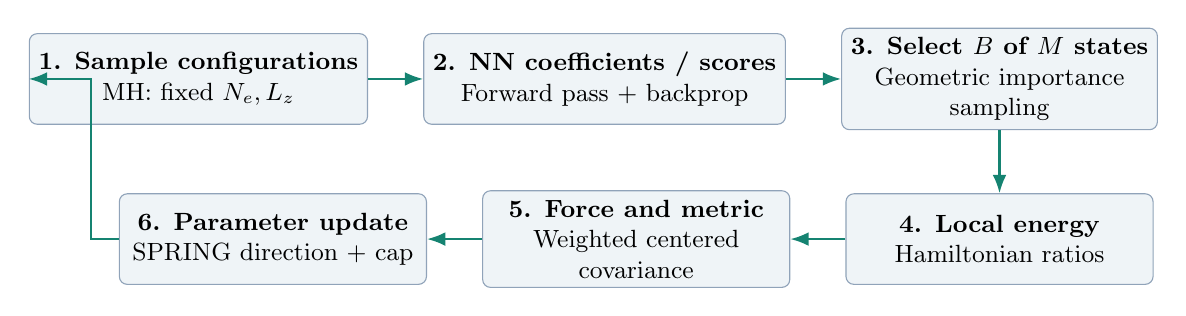
\begin{tikzpicture}[>=Latex,node distance=4mm and 7mm,
flowbox/.style={draw=blue!55,fill=pale,rounded corners=1mm,minimum width=3.9cm,minimum height=1.15cm,align=center,font=\small}]
\node[flowbox] (s) {\textbf{1. Sample configurations}\\MH: fixed $N_e,L_z$};
\node[flowbox,right=of s] (o) {\textbf{2. NN coefficients / scores}\\Forward pass + backprop};
\node[flowbox,right=of o] (b) {\textbf{3. Select $B$ of $M$ states}\\Geometric importance\\sampling};
\node[flowbox,below=8mm of b] (e) {\textbf{4. Local energy}\\Hamiltonian ratios};
\node[flowbox,left=of e] (g) {\textbf{5. Force and metric}\\Weighted centered\\covariance};
\node[flowbox,left=of g] (u) {\textbf{6. Parameter update}\\SPRING direction + cap};
\draw[->,thick,teal] (s)--(o);\draw[->,thick,teal] (o)--(b);\draw[->,thick,teal] (b)--(e);
\draw[->,thick,teal] (e)--(g);\draw[->,thick,teal] (g)--(u);
\draw[->,thick,teal] (u.west)--++(-.35,0)|-(s.west);
\end{tikzpicture}
\end{center}
\ml{minibatch generation $\rightarrow$ network/Jacobian evaluation $\rightarrow$ covariance-preconditioned parameter update.}\par\medskip
\textbf{Independent check:} freeze the network and compare complete-sector energy, variance and fidelity with ED.
\take{Every update generates new data. ED validates the frozen state without supplying training labels.}
\src{train\_exploration.py. Checkpoints store distinct neural parameters, raw SPRING direction memory, walkers and RNGs. These are updates, not fixed-dataset epochs; candidate sampling and update-batch selection are separate operations.}
\end{frame}

% 13
\begin{frame}{Logarithmic derivatives define the sampled tangent geometry}
\[
O_{ij}=\partial_{\theta_j}\log\psi_\theta(\nn_i)
=\partial_{\theta_j}a_\theta(\nn_i)+i\,\partial_{\theta_j}\varphi_\theta(\nn_i).
\]
\small For normalized weights $w_i$, center $\delta O_i=O_i-\sum_jw_jO_j$ and $\delta e_i=E_{{\rm loc},i}-\sum_jw_jE_{{\rm loc},j}$.
\[
A=\begin{pmatrix}\Re[\sqrt w\,\delta O]\\\Im[\sqrt w\,\delta O]\end{pmatrix},\qquad
e=\begin{pmatrix}\Re[\sqrt w\,\delta e]\\\Im[\sqrt w\,\delta e]\end{pmatrix},
\quad \widehat S=A^TA,\quad \widehat f=A^Te\approx\tfrac12\nabla_\theta E.
\]
\begin{columns}[T,onlytextwidth]
\column{.48\textwidth}
\begin{block}{What $O$ contains}
Every derivative through every hidden layer and readout. It is a Jacobian of the \emph{log wavefunction}, not the Hamiltonian matrix.
\end{block}
\column{.48\textwidth}
\begin{block}{What batch size controls}
$O:\ 32\times22,850$ complex; minimal $A:\ 64\times22,850$ real. Only a sampled tangent subspace is visible per update.
\end{block}
\end{columns}
\src{geometry\_sampling.py; JaQMC jasr.py. The weighted adapter uses signed duplicate rows and an actual $128\times128$ Gram solve, adding no independent information (backup). Both magnitude and phase derivatives are retained.}
\end{frame}

\section{Results and limits}
% 14
\begin{frame}{Ising checks the energy gradient and SPRING implementation}
\[
H_{\rm I}=-J\sum_i Z_iZ_{i+1}-h\sum_iX_i,\qquad N=6,\quad J=h=1.
\]
\begin{columns}[T,onlytextwidth]
\column{.68\textwidth}
\includegraphics[width=\linewidth,height=3.6cm,keepaspectratio]{slide_ising.pdf}
\column{.29\textwidth}
\small
\textbf{Periodic Pauli chain}\par\medskip
64 configurations; positive even-parity RBM, 12 hidden units, 73 parameters.\par\medskip
\textbf{After 250 updates}\par
$E-E_0=1.576\times10^{-5}J$\par
$\fidelity=99.999857\%$\par
$\mathrm{Var}(H)=2.054\times10^{-4}J^2$\par\smallskip
$E_0/J=-7.727406610$.
\end{columns}
\take{Independent exact Born draws and full-basis checks verify the energy gradient and SPRING adapter before fermionic tests.}
\src{SPRING\_Ising\_test saved run: batch 128, $\eta=.05$, $\lambda=.001$, $\mu=.9$, radius .1. Exact categorical sampling over 64 states, not MCMC. Gradient/autodiff maximum discrepancy $1.94\times10^{-15}$.}
\end{frame}

% 15
\begin{frame}{ED benchmarks the entire FQHE state}
\begin{columns}[T,onlytextwidth]
\column{.45\textwidth}
\textbf{Pure $V_1$, LLL sphere, $L_z=0$}\par\vspace{2mm}
\small\renewcommand{\arraystretch}{1.35}
\begin{tabular}{@{}rrrr@{}}\toprule
$N_e$ & $N_\phi$ & Orbitals & Sector states\\\midrule
4 &9&10&18\\5&12&13&73\\6&15&16&338\\7&18&19&1,656\\8&21&22&8,512\\\bottomrule
\end{tabular}
\par\medskip
Saved basis, sparse $H$, eigenpairs and manifests; no ED coefficients in the NN loss.
\column{.51\textwidth}
\textbf{A retained N=6 neural example}\par\smallskip
\small One width-64 hidden layer; 1,218 real parameters.\par
\[
E/V_1=0.0370740,\quad E_0\simeq0,\quad \fidelity=98.1674\%.
\]
\[
\mathrm{Var}(H)/V_1^2=0.105993.
\]
\small A selected best run from an earlier tuning set, using reweighted broader sampling. Accurate, but not exact.\par\medskip
\textbf{Validation metrics}\par
$\Delta E=E-E_0$, $\mathrm{Var}(H)=\|(H-E)\psi\|^2$,\\
$\fidelity=|\langle\psi_{\rm ED}|\psi_\theta\rangle|^2$.
\end{columns}
\take{Zero variance identifies an eigenstate; ground-state accuracy also needs the correct energy or ED overlap.}
\src{references/ne4--ne8 and results/ed\_benchmarks; retained N6: results/ne6\_baseline/original/best. Historical N6 and later N7/N8 runs use different protocols, so they are not a controlled size-scaling experiment.}
\end{frame}

% 16
\begin{frame}{Born-sampled SPRING already approaches the ED state}
\small $N_e=7$, six width-64 layers; original GG-SPRING with Born candidate pool ($\beta=1$).
\par\vspace{1mm}
\includegraphics[width=.98\textwidth,height=3.3cm,keepaspectratio]{slide_born_baseline.pdf}
\small\renewcommand{\arraystretch}{1.15}
\begin{center}
\begin{tabular}{@{}lrrrr@{}}\toprule
State / method & Mean $E/V_1$ & Mean $(E-E_0)/V_1$ & Mean fidelity & Mean variance$/V_1^2$\\\midrule
ED reference &2.82308&0&100\%&0\\
Original Born pool &2.97471&0.15162&91.28\%&0.37714\\\bottomrule
\end{tabular}
\end{center}
\take{SPRING reaches 91.28\% ED fidelity with Born sampling; broader sampling reaches 94.84\%.}
\src{Three-seed means at 10k; GG selection is retained. Same wall Hamiltonian as the broader-pool test: flux18, $U=10V_1$, $x_c=.88$, $L_z=0$. ED is the minimum within this sector. Curves join verified 8k parents and Born continuations; no ED training labels.}
\end{frame}

% 17
\begin{frame}{GG-SPRING: geometry-guided selection before the update}
\small GG adds a sample-selection stage to the existing SPRING optimizer; the physical energy loss is unchanged.
\begin{center}\vspace{-1mm}
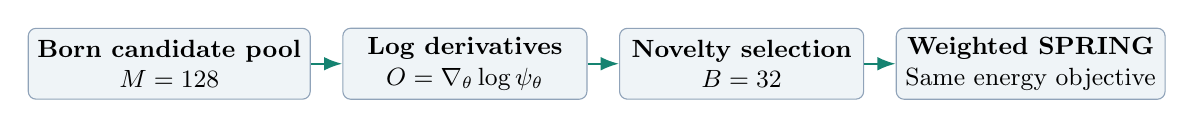
\begin{tikzpicture}[>=Latex,node distance=4mm,
ggbox/.style={draw=blue!55,fill=pale,rounded corners=1mm,minimum width=3.1cm,minimum height=.9cm,align=center,font=\small}]
\node[ggbox] (pool) {\textbf{Born candidate pool}\\$M=128$};
\node[ggbox,right=of pool] (score) {\textbf{Log derivatives}\\$O=\nabla_\theta\log\psi_\theta$};
\node[ggbox,right=of score] (select) {\textbf{Novelty selection}\\$B=32$};
\node[ggbox,right=of select] (update) {\textbf{Weighted SPRING}\\Same energy objective};
\draw[->,thick,teal] (pool)--(score);\draw[->,thick,teal] (score)--(select);\draw[->,thick,teal] (select)--(update);
\end{tikzpicture}
\end{center}
\begin{columns}[T,onlytextwidth]
\column{.57\textwidth}
\begin{itemize}\setlength\itemsep{4pt}
\item Scores describe how the variational wavefunction responds to a parameter change.
\item Center and scale the scores; compare with the previous selected batch, rescored at the current $\theta$.
\item Favor a larger out-of-span fraction $\nu_i\in[0,1]$, while retaining a uniform selection component.
\end{itemize}
\column{.39\textwidth}
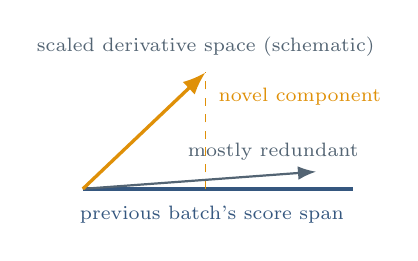
\begin{tikzpicture}[x=.78cm,y=.78cm,>=Latex]
\draw[blue,very thick] (0,0)--(4.4,0);
\node[blue,below] at (2.1,-.12) {\scriptsize previous batch's score span};
\draw[->,muted,thick] (0,0)--(3.8,.28);
\node[muted,above] at (3.1,.3) {\scriptsize mostly redundant};
\draw[->,orange,very thick] (0,0)--(2.0,1.9);
\draw[dashed,orange] (2.0,0)--(2.0,1.9);
\node[orange,right] at (2.05,1.5) {\scriptsize novel component};
\node[muted,above] at (2.0,2.0) {\scriptsize scaled derivative space (schematic)};
\end{tikzpicture}
\end{columns}
\[
\pi_i=\frac{0.2}{M}+0.8\frac{\nu_i+0.01}{\sum_j(\nu_j+0.01)},
\qquad w_i\propto\frac{1}{M\pi_i}.
\]
\take{Goal: more complementary tangent information in each update batch, with importance corrections for the selection.}
\src{Experimental project extension: geometry\_sampling.py. Uses diagonal-metric scaling and a ridge-smoothed projection; distances are between derivative responses, not Slater-state overlaps. Selection has full support and replacement; normalized weights retain finite-batch ratio/covariance bias. No ED labels enter selection.}
\end{frame}

% 18
\begin{frame}{N=7: geometric sampling and the wall target are separate tests}
\begin{columns}[T,onlytextwidth]
\column{.50\textwidth}
\textbf{No wall: 5k-update sampling comparison}\par\smallskip
\small Three-seed means; same six-layer network. Pool controls use $128\to32$ candidates.\par\vspace{2mm}
\renewcommand{\arraystretch}{1.3}
\begin{tabular}{@{}lrr@{}}\toprule
Method & $E/V_1$ & Fidelity\\\midrule
SPRING, batch 32 &1.24597&7.78\%\\
Random pool selection &1.12186&9.54\%\\
Geometry-guided (GG) &0.82157&16.40\%\\\bottomrule
\end{tabular}
\par\medskip
\small GG selects score directions that are novel relative to the previous batch, with inverse-probability weights.
\column{.46\textwidth}
\textbf{With wall: the 8k continuation parents}\par\smallskip
\small $U=10V_1$, $x_c=.88$; same $N_e=7$, flux18, $L_z=0$, 19 orbitals.\par
\[
E_0/V_1=2.823084663,
\]
\[
\overline{E-E_0}/V_1=0.154239,\qquad
\overline{\fidelity}=90.8512\%.
\]
\small The wall ED state has only \textbf{2.75\%} squared overlap with the no-wall Laughlin state.
\end{columns}
\take{The wall changes the target; its higher fidelity is not evidence of a better optimizer for the original Laughlin problem.}
\src{ne7\_gg\_spring\_20261111 (5k, no wall) and ne7\_gg\_edge\_20261111 (8k). Different Hamiltonians/budgets across the two panels. GG uses a diagonal-metric, ridge-smoothed novelty heuristic, not an exact full-QGT projection.}
\end{frame}

% 19
\begin{frame}{Rare configurations can dominate the residual error}
\vspace{1.2mm}
\includegraphics[width=.98\textwidth,height=3.8cm,keepaspectratio]{slide_rare.pdf}
\begin{columns}[T,onlytextwidth]
\column{.48\textwidth}
\small At the three wall 8k checkpoints, configurations with individual $p_\theta(\nn)<10^{-6}$ carry only $8\times10^{-6}$--$2.4\times10^{-5}$ total Born mass.
\column{.48\textwidth}
\small Yet they contain \textbf{90--98\% of the exact residual variance}. A quiet batch variance can therefore coexist with a substantial exact error.
\end{columns}
\take{Geometric selection cannot choose a useful configuration that never entered the candidate pool. Low probability alone, however, does not imply importance.}
\src{Frozen complete-sector diagnostics in ne7\_gg\_explore\_20261111/frozen\_probe.json. Coverage probabilities here assume independent candidate draws; persistent training chains also have autocorrelation/equilibration error.}
\end{frame}

% 20
\begin{frame}{Broaden the proposal, then reweight to the physical objective}
\begin{columns}[T,onlytextwidth]
\column{.54\textwidth}
\[
q_\beta(\nn)\propto|\psi_\theta(\nn)|^{2\beta},\qquad \beta=0.5.
\]
\small If draw $t$ selects candidate index $i$ with conditional probability $\pi_t(i)>0$,
\[
\widetilde w_t=\frac{|\psi_\theta(\nn_i)|^{2(1-\beta)}}{M\pi_t(i)},\qquad
w_t=\frac{\widetilde w_t}{\sum_s\widetilde w_s}.
\]
\small The two factors correct the broader proposal and the geometric selection. The physical Hamiltonian and energy objective stay fixed.
\column{.42\textwidth}
\textbf{Three paired branches from each 8k state}\par\medskip
\begin{enumerate}\setlength\itemsep{5pt}
\item Original GG: Born pool, static novelty.
\item Broader pool: $\beta=.5$, static novelty.
\item Broader + sequential geometry: update the selected score span after each draw.
\end{enumerate}
\small Same $M=128$, $B=32$, network, optimizer and Hamiltonian; 2k added updates per branch.
\end{columns}
\take{This is sampling broadening, not a physical temperature or a cooling schedule. It is a testable intervention rather than a convergence guarantee.}
\src{Full SPRING memory/counters, parameters and RNGs restored. Hot pools receive 500 frozen-parameter warmup sweeps. Full-support selection with replacement is retained. Self-normalized ratios/covariances have finite-batch bias; importance weights can reduce ESS.}
\end{frame}

% 21
\begin{frame}{Broader sampling improves accuracy at nearly the same cost}
\vspace{1.2mm}
\includegraphics[width=.98\textwidth,height=3.5cm,keepaspectratio]{slide_broad.pdf}
\vspace{-1mm}
\small\renewcommand{\arraystretch}{1.15}
\begin{center}
\begin{tabular}{@{}lrrrr@{}}\toprule
Method & Mean $(E-E_0)/V_1$ & Mean fidelity & Mean variance$/V_1^2$ & Mean active s\\\midrule
Original GG &0.15162&91.28\%&0.37714&28.6\\
Broader pool &0.09836&94.84\%&0.25147&29.5\\
Broader + sequential &0.09627&95.22\%&0.24429&57.1\\\bottomrule
\end{tabular}
\end{center}
\small
\textbf{Broader pool:} 35\% less mean energy error for 3\% more active time; improves all three seeds.\par
\textbf{Sequential addition:} 2.1\% further mean error reduction, 1.94$\times$ time; lower energy in only 1/3 seeds.
\src{ne7\_gg\_explore\_20261111: all 9 runs and 45 full-sector ED evaluations validated. Three paired learned states, not a universal optimizer ranking. Best fidelity 98.76\%; difficult seed remains 89.2\%. Active times exclude compilation, frozen warmup and ED; no ground-state convergence claim.}
\end{frame}

\appendix
\section{Reference and technical backup}
% 22
\begin{frame}{References and the scope of the comparison}
\footnotesize
\begin{enumerate}\setlength\itemsep{5pt}
\item F. D. M. Haldane, \emph{Fractional quantization of the Hall effect: A hierarchy of incompressible quantum fluid states}, PRL 51, 605 (1983). \href{https://doi.org/10.1103/PhysRevLett.51.605}{doi:10.1103/PhysRevLett.51.605}.
\item R. B. Laughlin, \emph{Anomalous quantum Hall effect: An incompressible quantum fluid with fractionally charged excitations}, PRL 50, 1395 (1983). \href{https://doi.org/10.1103/PhysRevLett.50.1395}{doi:10.1103/PhysRevLett.50.1395}.
\item G. Carleo and M. Troyer, \emph{Solving the quantum many-body problem with artificial neural networks}, Science 355, 602 (2017). \href{https://arxiv.org/abs/1606.02318}{arXiv:1606.02318}.
\item A. Chen and M. Heyl, \emph{Empowering deep neural quantum states through efficient optimization}, Nature Physics 20, 1476 (2024). \href{https://arxiv.org/abs/2302.01941}{arXiv:2302.01941}.
\item G. Goldshlager, N. Abrahamsen and L. Lin, \emph{A Kaczmarz-inspired approach to accelerate the optimization of neural network wavefunctions}, JCP 516, 113351 (2024). \href{https://arxiv.org/abs/2401.10190}{arXiv:2401.10190}.
\item Y. Teng, D. D. Dai and L. Fu, \emph{Solving and visualizing fractional quantum Hall wavefunctions with neural network}, PRB 111, 205117 (2025). \href{https://arxiv.org/abs/2412.00618}{arXiv:2412.00618}.
\end{enumerate}
\take{The molecular SPRING--MinSR/KFAC ranking is literature evidence. Our latest FQHE comparison holds SPRING fixed and varies sampling/selection.}
\src{[6] uses a disk, real-space attention FNN and allows Landau-level mixing; this project uses a strictly LLL sphere occupation MLP. Internal data/source pointers and figure input hashes are retained beside this deck.}
\end{frame}

% 23
\begin{frame}{Backup: complex geometry and implementation dimensions}
\begin{columns}[T,onlytextwidth]
\column{.55\textwidth}
\small
For $P$ real parameters and $B$ complex score rows, the batch estimators are
\[
\widehat S_{jk}=\Re\sum_iw_i\,\delta O_{ij}^*\delta O_{ik},\qquad
\widehat f_j=\Re\sum_iw_i\,\delta O_{ij}^*\delta e_i.
\]
The weighted adapter supplies signed rows
\[
J=\begin{bmatrix}+\sqrt{Bw}\,\delta O\\-\sqrt{Bw}\,\delta O\end{bmatrix}
\in\mathbb C^{2B\times P}.
\]
JaQMC normalization and realification preserve $S$ while producing $4B$ real rows. Thus $B=32$ gives an actual \textbf{$128\times128$} Gram solve. Signed copies add no information; the rank is at most $2(B-1)=62$ before further redundancies.
\column{.41\textwidth}
\textbf{22,850 real parameters}\par\small
\begin{align*}
P={}&(19\cdot64+64)\\
&+5(64^2+64)\\
&+6(64\cdot2)+2\\
={}&22,850.
\end{align*}
\textbf{Sign convention}\par\smallskip
Code stores positive-force direction $d$ and applies $-\alpha d$.\par\smallskip
Paper-style descent direction $\phi=-d$ uses $\epsilon=-e$ and update $+\alpha\phi$. These are equivalent.
\end{columns}
\src{Sphere spinor gauge: $u=\cos(\vartheta/2)e^{i\phi/2}$, $v=\sin(\vartheta/2)e^{-i\phi/2}$. Adapter: geometry\_sampling.py and JaQMC jasr.py. Known centered mean-null directions are lifted for stable Cholesky without changing the exact-arithmetic centered update.}
\end{frame}
\end{document}
